\chapter{RESULTADOS ESPERADOS\label{resultados_esperados}}

\hspace*{1.25cm}Nesta Se��o s�o demonstradas algumas imagens que
representam os resultados finais esperados.

\hspace*{0.65cm}A Figura \ref{img:resultados_preview1}, representa a
a��o do sistema em resposta da inser��o de um novo v�deo pelo
editor, oferecendo a op��o de detectar as transi��es naquele momento
(pressionando ``OK'') ou somente posteriormente (pressionando
``Cancel'').

\begin{figure}[h|top]
 \centering
 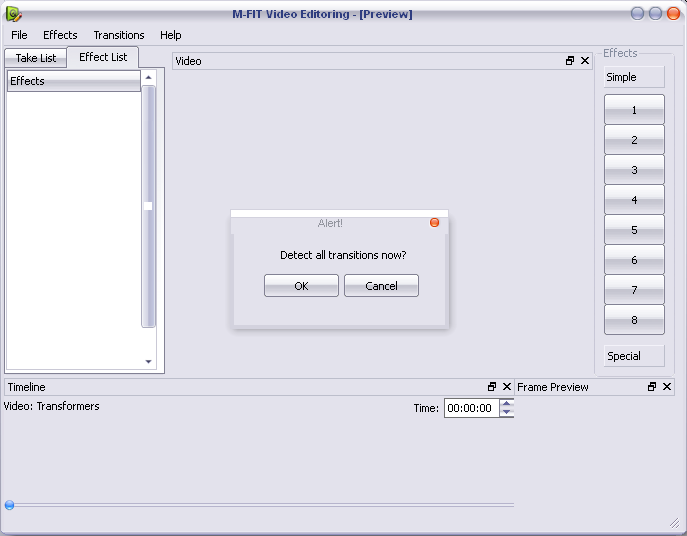
\includegraphics[width=1.0\linewidth]{imagens/resultados_preview1.png}
 \caption{Interface de abertura de um novo V�deo.}
 Fonte: Autor.
 \label{img:resultados_preview1}
\end{figure}

\hspace*{0.65cm}Se a op��o de escolha for o ``Cancel'', o sistema
n�o far� a detec��o das transi��es, e a �rea de trabalho do editor
ser� aberta com alguns elementos faltantes. O editor poder� a
qualquer momento desejar que as transi��es sejam detectadas. Para
isso � feito o acesso do menu "Transition" e escolhendo que tipo de
transi��o ele deseja que seja detectado. Este tipo de procedimento
pode ser realizado caso o editor queira detectar somente transi��es
do tipo corte. Este exemplo pode ser verificado na Figura
\ref{img:resultados_preview2}.

\begin{figure}[h|top]
 \centering
 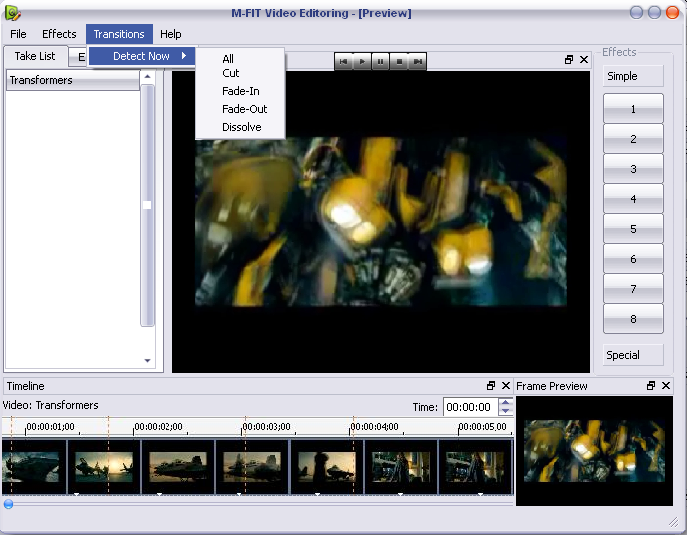
\includegraphics[width=1.0\linewidth]{imagens/resultados_preview2.png}
 \caption{Area de trabalho sem ter as transi��es detectadas.}
 Fonte: Autor.
 \label{img:resultados_preview2}
\end{figure}

\hspace*{0.65cm}Se a op��o de escolha foi o ``OK'', o sistema
realizar� a detec��o de todas as transi��es do v�deo. A partir
disso, ir� gerar uma lista com todas as tomadas do v�deo. O editor
ent�o, tem a possibilidade de selecionar uma das v�rias tomadas da
lista, delimitando-as assim na timeline. Esta vis�o pode ser
visualizada na Figura \ref{img:resultados_preview3}.

\begin{figure}[h|top]
 \centering
 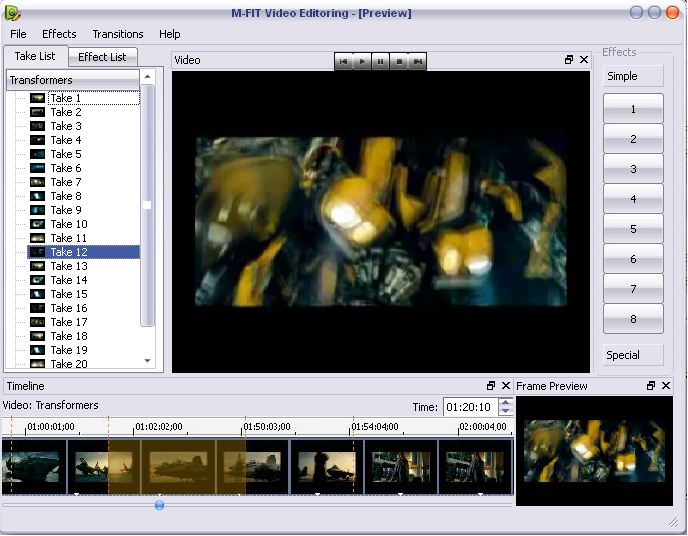
\includegraphics[width=1.0\linewidth]{imagens/resultados_preview3.png}
 \caption{Area de trabalho com as transi��es detectadas.}
 Fonte: Autor.
 \label{img:resultados_preview3}
\end{figure}
